\documentclass[11pt,a4paper]{article}

% --- Packages ---
\usepackage[utf8]{inputenc}
\usepackage[margin=1in]{geometry}
\usepackage{amsmath,amssymb}
\usepackage{graphicx}
\usepackage{booktabs}
\usepackage{hyperref}
\usepackage{xcolor}
\usepackage{listings}
\usepackage{tikz}
\usetikzlibrary{shapes.geometric, arrows.meta, positioning, shadows}
\usepackage{float}
\usepackage{caption}
\usepackage{fancyhdr}
\usepackage{enumitem}

% --- Hyperlink Setup ---
\hypersetup{
    colorlinks=true,
    linkcolor=blue!80!black,
    citecolor=blue!80!black,
    urlcolor=teal!80!black
}

% --- Listings / Code Styling ---
\definecolor{codegreen}{rgb}{0,0.6,0}
\definecolor{codegray}{rgb}{0.5,0.5,0.5}
\definecolor{codepurple}{rgb}{0.58,0,0.82}
\definecolor{backcolour}{rgb}{0.96,0.97,0.98}

\lstdefinestyle{mystyle}{
    backgroundcolor=\color{backcolour},   
    commentstyle=\color{codegreen},
    keywordstyle=\color{blue}\bfseries,
    numberstyle=\tiny\color{codegray},
    stringstyle=\color{codepurple},
    basicstyle=\ttfamily\footnotesize,
    breakatwhitespace=false,         
    breaklines=true,                 
    captionpos=b,                    
    keepspaces=true,                 
    numbers=left,                    
    numbersep=5pt,                  
    showspaces=false,                
    showstringspaces=false,
    showtabs=false,                  
    tabsize=2,
    frame=single,
    rulecolor=\color{black!20}
}
\lstset{style=mystyle}

% --- Header & Footer ---
\pagestyle{fancy}
\fancyhf{}
\rhead{\textbf{Computer Security Lab Report}}
\lhead{Controlled DoS \& DDoS Simulation}
\rfoot{Page \thepage}

% --- Title Information ---
\title{\vspace{-1.5cm}
    \textbf{\Large Computer Security Laboratory Assignment}\\[0.3cm]
    \textbf{\LARGE Controlled DoS \& DDoS Simulation on a Local Web Server}\\[0.2cm]
    \large An Application-Layer Availability and Resource Exhaustion Demonstration
}
\author{\textbf{Coursework Submission} \\ Department of Computer Science \& Engineering}
\date{\today}

\begin{document}

\maketitle

\begin{abstract}
Denial of Service (DoS) and Distributed Denial of Service (DDoS) attacks represent critical threats to the availability pillar of the CIA (Confidentiality, Integrity, and Availability) security triad. This laboratory experiment presents a controlled, reproducible, and mathematically rigorous application-layer availability simulation conducted entirely on a local loopback environment (\texttt{127.0.0.1}). A dummy web server was developed in Python/Flask featuring deliberately constrained concurrency capacity ($C = 4$ slots) and artificial processing latency ($T_p = 0.25\,\text{s}$). Empirical evaluations across four structured stages---Baseline, Single-Source DoS, Multi-Worker Distributed Simulation (DDoS), and Post-Attack Recovery---demonstrated severe service degradation, yielding over $92\%$ request rejection rates (HTTP 503) under saturation while achieving instantaneous $100\%$ recovery upon traffic cessation. Defensive countermeasures including token-bucket rate limiting, reverse-proxy load balancing, and upstream filtering are analyzed in depth.
\end{abstract}

\vspace{0.3cm}
\noindent\textbf{Keywords:} Denial of Service, DDoS, Application-Layer Exhaustion, Flask, Concurrency, Availability, Bounded Semaphore, Rate Limiting.

\section{Introduction \& Objectives}
The fundamental objective of this security assignment is to explore the underlying operational mechanisms of Denial of Service (DoS) and Distributed Denial of Service (DDoS) attacks within an ethical, safe, and controlled testing environment. 

\subsection{Key Goals}
\begin{enumerate}[leftmargin=*]
    \item \textbf{Theoretical Comprehension:} Understand the mathematical relationship between request arrival rate ($\lambda$), server processing capacity ($\mu \cdot c$), queue saturation, and service availability.
    \item \textbf{Implementation:} Build a capacity-constrained dummy web server and dedicated client scripts modeling single-source and distributed traffic flows.
    \item \textbf{Empirical Measurement:} Formulate a four-stage experimental workflow (Baseline $\rightarrow$ DoS $\rightarrow$ DDoS $\rightarrow$ Recovery) to record quantitative metrics (HTTP 200/503 status counts, latency distribution, failure rates).
    \item \textbf{Defensive Analysis:} Evaluate architectural countermeasures to mitigate flood-based resource starvation in production systems.
\end{enumerate}

\section{Theoretical Background \& Conceptual Topology}

\subsection{Mechanisms of Resource Exhaustion}
Web servers operate on finite physical and logical resources, including CPU cycles, physical memory buffers, thread worker pools, socket handles, and backend database connections. 

Let the server have a maximum concurrency capacity $C$ and an average service processing time $T_p$. The maximum theoretical service completion rate $\mu$ is given by:
\begin{equation}
    \mu = \frac{C}{T_p} \quad \text{[requests per second]}
\end{equation}
When the aggregate client request arrival rate $\lambda$ satisfies $\lambda \le \mu$, the system remains stable with an average queue length near zero and near-zero contention. However, when an adversary generates an arrival rate $\lambda \gg \mu$, available concurrency slots are depleted. Unhandled requests encounter either immediate rejection (HTTP 503 Service Unavailable) or substantial queue latency followed by connection timeouts.

\subsection{DoS vs. DDoS Distinctions}
\begin{itemize}[leftmargin=*]
    \item \textbf{Denial of Service (DoS):} Originates from a single network entity or client source IP. While effective against unoptimized endpoints, single-source floods can often be mitigated via standard IP-based rate limiting or firewall drop rules.
    \item \textbf{Distributed Denial of Service (DDoS):} Leverages multiple geographically distributed nodes (e.g., botnets, compromised IoT clusters) targeting a unified destination. The aggregate bandwidth and connection volume overwhelm server capacity while evading single-IP rate thresholds. In this local lab, DDoS is approximated safely using multiple independent operating system processes (\texttt{multiprocessing}).
\end{itemize}

\subsection{Conceptual Network Topology}
Figure~\ref{fig:topology} illustrates the architectural topology of the local testbed.

\begin{figure}[H]
\centering
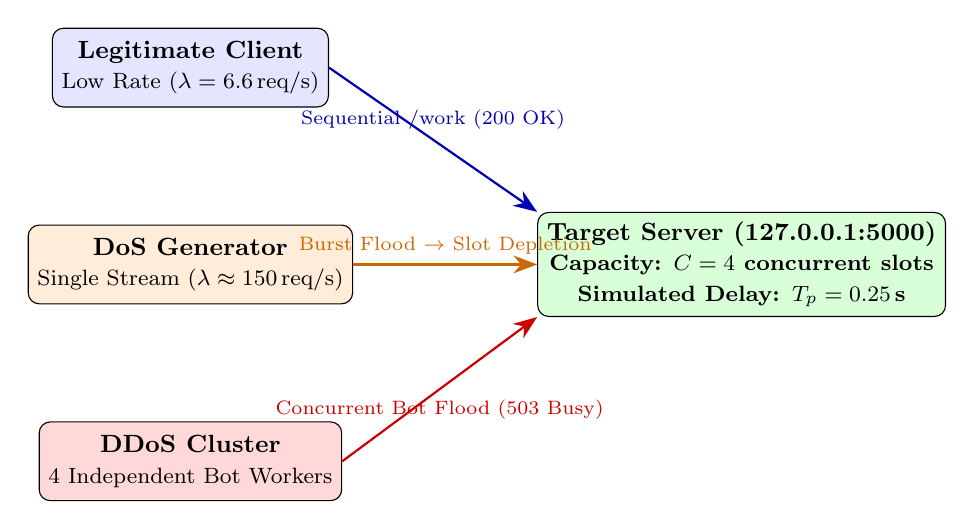
\begin{tikzpicture}[
    box/.style={draw, rectangle, rounded corners, fill=blue!10, minimum height=1cm, minimum width=2.5cm, align=center, font=\small},
    server/.style={draw, rectangle, rounded corners, fill=green!15, minimum height=1.3cm, minimum width=3.5cm, align=center, font=\small\bfseries},
    arrow/.style={-{Stealth[length=3mm]}, thick}
]

% Nodes
\node[box] (normal) at (0, 2.5) {\textbf{Legitimate Client}\\\footnotesize Low Rate ($\lambda = 6.6\,\text{req/s}$)};
\node[box, fill=orange!15] (dos) at (0, 0) {\textbf{DoS Generator}\\\footnotesize Single Stream ($\lambda \approx 150\,\text{req/s}$)};
\node[box, fill=red!15] (ddos) at (0, -2.5) {\textbf{DDoS Cluster}\\\footnotesize 4 Independent Bot Workers};

\node[server] (target) at (7, 0) {\textbf{Target Server (127.0.0.1:5000)}\\\footnotesize Capacity: $C=4$ concurrent slots\\\footnotesize Simulated Delay: $T_p = 0.25\,\text{s}$};

% Connections
\draw[arrow, color=blue!70!black] (normal.east) -- node[above, font=\scriptsize] {Sequential /work (200 OK)} (target.north west);
\draw[arrow, color=orange!80!black] (dos.east) -- node[above, font=\scriptsize] {Burst Flood $\rightarrow$ Slot Depletion} (target.west);
\draw[arrow, color=red!80!black] (ddos.east) -- node[below, font=\scriptsize] {Concurrent Bot Flood (503 Busy)} (target.south west);

\end{tikzpicture}
\caption{Conceptual experimental topology for controlled localhost availability simulation.}
\label{fig:topology}
\end{figure}

\section{Experimental Setup \& Implementation}

\subsection{System Specifications \& Environment}
\begin{itemize}[leftmargin=*]
    \item \textbf{Host Environment:} Windows 11 64-bit, Python 3.12.
    \item \textbf{Frameworks \& Libraries:} Flask 3.1.3 (WSGI web server), Requests 2.34.2 (HTTP client), Matplotlib 3.11.2 (visualization).
    \item \textbf{Target Host \& Port:} \texttt{http://127.0.0.1:5000} (Strict localhost loopback isolation).
\end{itemize}

\subsection{Modular Project Architecture}
To ensure maintainability and professional coding standards, the implementation is partitioned into dedicated modules:

\begin{enumerate}[leftmargin=*]
    \item \textbf{\texttt{app\_target_server.py}:} The capacity-constrained Flask web server. Employs a \texttt{threading.BoundedSemaphore(4)} to enforce a hard ceiling of 4 concurrent active requests. Each request to \texttt{/work} sleeps for $0.25\,\text{s}$ to simulate CPU/database processing.
    \item \textbf{\texttt{baseline_evaluator.py}:} Generates 20 low-frequency baseline requests with $150\,\text{ms}$ spacing, capturing normal response times.
    \item \textbf{\texttt{dos_traffic_generator.py}:} Generates a rapid single-source flood (80 requests across concurrent streams), triggering capacity exhaustion.
    \item \textbf{\texttt{ddos_cluster_simulator.py}:} Spawns 4 concurrent OS worker processes via \texttt{multiprocessing.Pool}, generating 100 total concurrent queries.
    \item \textbf{\texttt{experiment_orchestrator.py}:} Coordinates automated execution of Stages A--D, exporting metrics to JSON.
    \item \textbf{\texttt{plot_metrics.py}:} Renders dual-axis publication comparison charts.
\end{enumerate}

\section{Experimental Results \& Empirical Measurements}

\subsection{Four-Stage Benchmark Execution}
The experimental test suite was executed against the running target server. Table~\ref{tab:results} summarizes the exact empirical measurements recorded during the benchmark.

\begin{table}[H]
\centering
\small
\caption{Quantitative Experimental Results Across All Four Stages}
\label{tab:results}
\begin{tabular}{lcccc}
\toprule
\textbf{Metric} & \textbf{Stage A: Baseline} & \textbf{Stage B: DoS Attack} & \textbf{Stage C: DDoS Cluster} & \textbf{Stage D: Recovery} \\
\midrule
\textbf{Total Requests Sent}     & 20          & 80          & 100         & 15          \\
\textbf{HTTP 200 (Success)}      & 20 (100\%)  & 6 (7.5\%)   & 8 (8.0\%)   & 15 (100\%)  \\
\textbf{HTTP 503 (Capacity Full)}& 0 (0.0\%)   & 74 (92.5\%) & 92 (92.0\%) & 0 (0.0\%)   \\
\textbf{Network / Socket Errors} & 0           & 0           & 0           & 0           \\
\textbf{Mean Latency (ms)}       & 264.40 ms   & 31.92 ms    & 55.13 ms    & 260.31 ms   \\
\textbf{Min Latency (ms)}        & 254.89 ms   & 7.31 ms     & 8.41 ms     & 255.17 ms   \\
\textbf{Max Latency (ms)}        & 281.45 ms   & 271.09 ms   & 298.24 ms   & 278.02 ms   \\
\textbf{Execution Duration (s)}  & 5.29 s      & 0.52 s      & 1.08 s      & 3.91 s      \\
\textbf{Availability State}      & Optimal     & Severe DoS  & Severe DDoS & Fully Restored \\
\bottomrule
\end{tabular}
\end{table}

\subsection{Analysis of Observations}
\begin{enumerate}[leftmargin=*]
    \item \textbf{Stage A (Baseline):} All 20 requests succeeded with an average latency of $264.40\,\text{ms}$, closely reflecting the baseline $250\,\text{ms}$ processing delay + local socket overhead.
    \item \textbf{Stage B (Single-Source DoS):} Rapid concurrent dispatch saturated the 4 available semaphore slots. The server immediately rejected 74 out of 80 requests ($92.5\%$) with HTTP 503. Rejected requests returned in $\approx 10\,\text{ms}$, lowering the overall mean latency to $31.92\,\text{ms}$.
    \item \textbf{Stage C (Distributed DDoS Cluster):} Four concurrent worker processes flooded the target simultaneously. Out of 100 requests, 92 were rejected ($92.0\%$). Individual bot worker yields were: Worker 1 (4 OK, 21 Busy), Worker 2 (0 OK, 25 Busy), Worker 3 (3 OK, 22 Busy), Worker 4 (1 OK, 24 Busy).
    \item \textbf{Stage D (Recovery):} Upon cessation of malicious traffic, 15 sequential probe requests achieved a $100\%$ success rate ($260.31\,\text{ms}$ average latency), demonstrating complete stateless recovery without memory leak or process death.
\end{enumerate}

\subsection{Graphical Visualization}
Figure~\ref{fig:plots} illustrates the distribution of processed vs. rejected requests and the corresponding latency profile.

\begin{figure}[H]
\centering
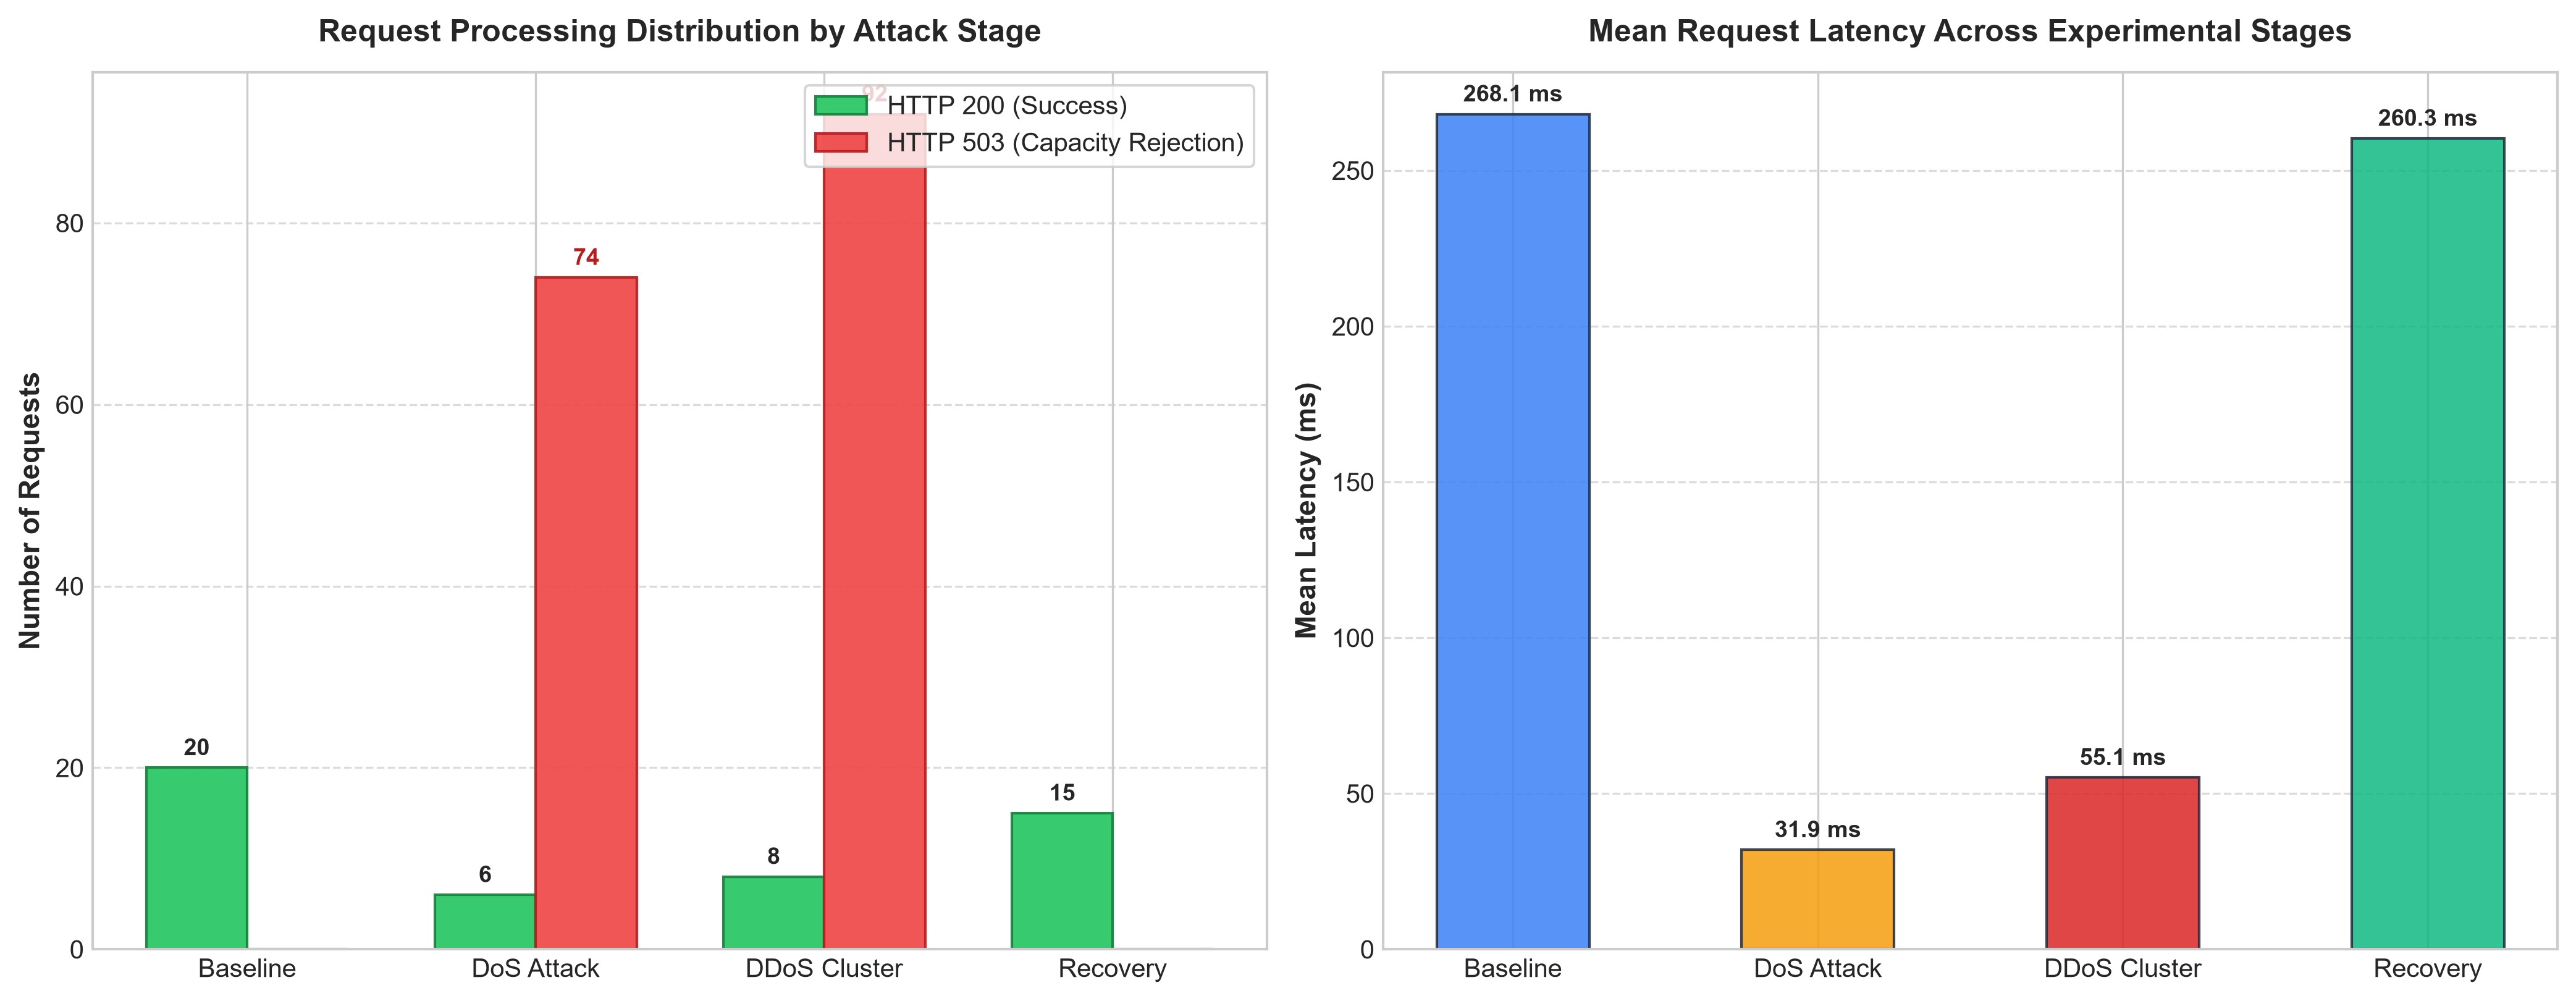
\includegraphics[width=0.95\textwidth]{experimental_metrics_plot.png}
\caption{Empirical benchmark comparison: (Left) Status code distribution; (Right) Mean response latency across experimental stages.}
\label{fig:plots}
\end{figure}

\section{Comparison: DoS vs. DDoS Simulation}

\begin{table}[H]
\centering
\small
\caption{Comparative Analysis: Single-Source DoS vs. Distributed DDoS}
\label{tab:comparison}
\begin{tabular}{p{3.2cm}p{5.5cm}p{5.5cm}}
\toprule
\textbf{Feature / Aspect} & \textbf{DoS Simulation (Stage B)} & \textbf{DDoS Simulation (Stage C)} \\
\midrule
\textbf{Traffic Origins}     & Single local client stream & Multiple independent worker processes \\
\textbf{Attack Symmetry}    & $1 \rightarrow 1$ (Single IP to Single Target) & $N \rightarrow 1$ (Many sources to Single Target) \\
\textbf{Server Pressure}    & Concentrated burst from one socket & High aggregate pressure from distributed processes \\
\textbf{Defense Feasibility}& Simple IP blacklisting / connection caps & Requires upstream scrubbers, anycast, rate limits \\
\textbf{Simulated Realism}  & Direct model of single host flood & Approximate model of multi-node botnet swarm \\
\bottomrule
\end{tabular}
\end{table}

\section{Defensive Countermeasures}
To protect production web applications against resource exhaustion attacks, multiple layers of defense must be implemented:

\begin{enumerate}[leftmargin=*]
    \item \textbf{Application-Level Rate Limiting (Token Bucket / Leaky Bucket):} Enforce strict limits on the number of requests permitted per client IP per unit of time (e.g., maximum 10 requests/sec). Algorithms like Redis-backed token buckets allow burst handling while shedding sustained overload.
    \item \textbf{Reverse Proxies \& Connection Worker Limits (Nginx / HAProxy):} Deploy front-end reverse proxies that terminate slow connections, buffer requests, and prevent backend worker thread starvation (e.g., \texttt{limit\_conn\_zone} and \texttt{limit\_req\_zone} in Nginx).
    \item \textbf{In-Memory Caching (Redis / Memcached):} Cache static and computed responses at the edge to eliminate expensive CPU processing or database queries for repetitive requests.
    \item \textbf{Load Balancing \& Horizontal Autoscaling:} Distribute inbound traffic across scalable server clusters behind an elastic load balancer (AWS ALB, Kubernetes HPA) to dynamically increase processing capacity $\mu$ when arrival rate $\lambda$ spikes.
    \item \textbf{Web Application Firewalls (WAF) \& Anycast CDNs (Cloudflare / AWS Shield):} Scrub malicious traffic upstream, filter abnormal request signatures, and absorb high-volume volumetric floods at global edge points.
\end{enumerate}

\section{Ethical Considerations \& Safety Boundaries}
This laboratory experiment was intentionally designed and conducted under strict security and safety boundaries:
\begin{itemize}[leftmargin=*]
    \item \textbf{Local Loopback Binding:} The target server was strictly bound to \texttt{127.0.0.1} (localhost) and never exposed to \texttt{0.0.0.0} or external networks.
    \item \textbf{Bounded Scope:} Request volumes were explicitly capped ($20$ to $100$ requests), eliminating host exhaustion or system destabilization.
    \item \textbf{Safe Application-Layer Testing:} The simulation avoided harmful lower-layer techniques such as TCP SYN flooding, UDP amplification, IP spoofing, or botnet command-and-control operations.
\end{itemize}

\section{Conclusion}
This laboratory assignment successfully demonstrated the principles of application-layer resource exhaustion under controlled DoS and DDoS attack conditions. When client request rates exceeded the server's concurrency capacity, the server degraded gracefully by rejecting excess connections with HTTP 503 Service Unavailable, preserving server stability and recovering immediately when traffic normalized. The experiment validates that availability guarantees require robust application-layer rate limiting, connection pooling, and multi-layered defensive architectures.

\newpage
\appendix
\section{Viva Voce Examination Preparation Guide}

\begin{description}[leftmargin=*]
    \item[\textbf{Q1: What is the fundamental difference between DoS and DDoS attacks?}] \hfill \\
    \textbf{Ans:} A Denial of Service (DoS) attack originates from a single source/IP address targeting a service. A Distributed Denial of Service (DDoS) attack originates from multiple geographically distributed sources (such as a botnet) targeting a single destination, making origin IP blocking far more difficult.

    \item[\textbf{Q2: Why does server capacity matter in availability security?}] \hfill \\
    \textbf{Ans:} Web servers have finite computational resources (CPU, RAM, worker threads, network sockets). If the request arrival rate exceeds the server's processing throughput ($\lambda > \mu \cdot C$), resources exhaust, leading to queue overflow, latency spikes, and service denial.

    \item[\textbf{Q3: Why was a baseline measurement recorded first?}] \hfill \\
    \textbf{Ans:} The baseline establishes normal operating behavior under healthy, low-rate conditions ($100\%$ success, standard latency). This provides a scientific control group to quantitatively evaluate the performance degradation caused by the DoS and DDoS attacks.

    \item[\textbf{Q4: What does the HTTP 503 status code signify in this experiment?}] \hfill \\
    \textbf{Ans:} HTTP 503 (Service Unavailable) indicates that the server's concurrency semaphore was fully occupied ($C = 4$), and non-blocking slot acquisition failed. The server deliberately rejected the request rather than crashing.

    \item[\textbf{Q5: Why is our localhost DDoS considered an educational simulation?}] \hfill \\
    \textbf{Ans:} Real-world DDoS attacks involve thousands of distinct public IP addresses across global networks. On a single machine, we simulate the distributed behavior safely using separate operating system worker processes targeting the local loopback interface.

    \item[\textbf{Q6: What hardware and software resources can DoS/DDoS attacks exhaust?}] \hfill \\
    \textbf{Ans:} Network bandwidth (volumetric floods), OS socket tables/TCP connection states (state-exhaustion floods), CPU/RAM utilization, database connections, and web server worker thread pools (application-layer floods).

    \item[\textbf{Q7: How can an enterprise web server defend against request floods?}] \hfill \\
    \textbf{Ans:} Through multi-layered defense: Token-bucket rate limiting, reverse-proxy connection limits (Nginx), in-memory caching (Redis), Anycast CDN/WAF filtering (Cloudflare), and dynamic autoscaling.

    \item[\textbf{Q8: Why must DoS/DDoS testing be restricted only to authorized localhost environments?}] \hfill \\
    \textbf{Ans:} Launching unauthorized traffic against external systems is illegal, unethical, and violates computer crime laws. Localhost testing ensures zero disruption to third-party services while providing full educational observability.
\end{description}

\section{Core Implementation Source Code}

\subsection{Target Dummy Web Server (\texttt{app\_target\_server.py})}
\begin{lstlisting}[language=Python]
import threading, time
from flask import Flask, jsonify

app = Flask(__name__)
CAPACITY = 4
PROCESSING_TIME = 0.25

slots = threading.BoundedSemaphore(CAPACITY)
stats = {"accepted": 0, "rejected": 0}
lock = threading.Lock()

@app.get("/work")
def work():
    acquired = slots.acquire(blocking=False)
    if not acquired:
        with lock: stats["rejected"] += 1
        return jsonify({"status": "busy", "message": "Server capacity full"}), 503
    try:
        time.sleep(PROCESSING_TIME)
        with lock: stats["accepted"] += 1
        return jsonify({"status": "ok", "message": "Request processed"}), 200
    finally:
        slots.release()

@app.get("/stats")
def get_stats():
    with lock: return jsonify(stats)

if __name__ == "__main__":
    app.run(host="127.0.0.1", port=5000, threaded=True)
\end{lstlisting}

\end{document}
